\newpage
\section{Resultados}
\indent Para probar el protocolo, armamos archivos de 1kb, 5kb, 10kb, 50kb, 100kb, 200kb y
500kb. El servidor y el cliente se encuentran en distintos host en la misma LAN sobre Wi-Fi la cual presenta un RTT de aproximadamente 2ms entre ambos hosts. Para
tomar los tiempos y comprobar el correcto funcionamiento del protocolo, usamos
el wireshark.\\
\indent Para tener mediciones mas aproximadas a la realidad, tomamos el promedio de 10 mediciones.\\

\subsection{Análisis del tiempo de transmisión}
\indent En este primer gráfico presentamos el tiempo de transmisión de los archivos, usando SEND\_WINDOWs de 1, 10, 15 y 20.

\begin{figure}[h]
  \centering                                                       
          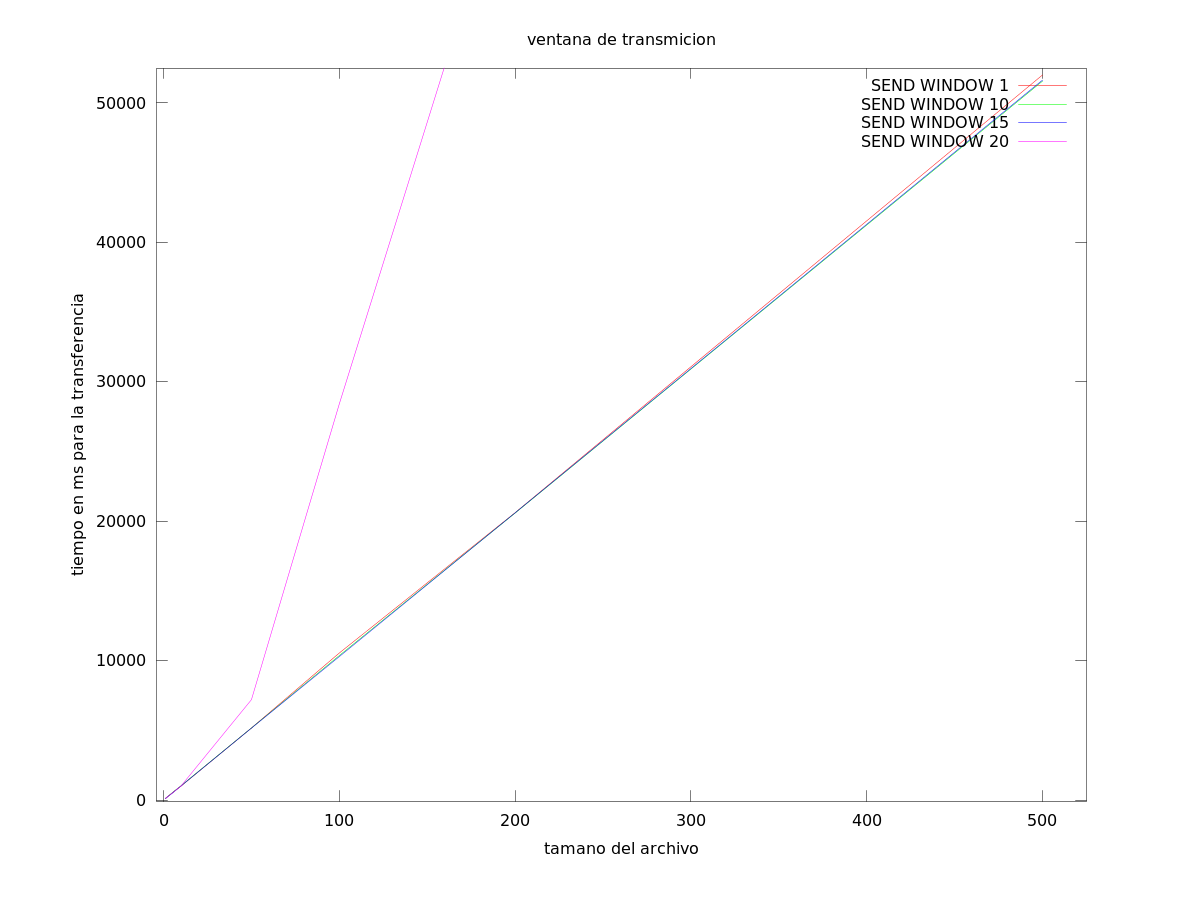
\includegraphics[width=500pt]{./datos/graf.png}
          \caption{Tiempo de transmisión}
          \label{fig:tt}
\end{figure}

\clearpage

\subsection{Velocidad de Transferencia}
\indent En este segundo gráfico presentamos la velocidad de transmisión (en kb\/s) de la transmisión de los archivos, usando SEND\_WINDOWs de 1, 10, 15 y 20.

\begin{figure}[h]
  \centering                                                       
          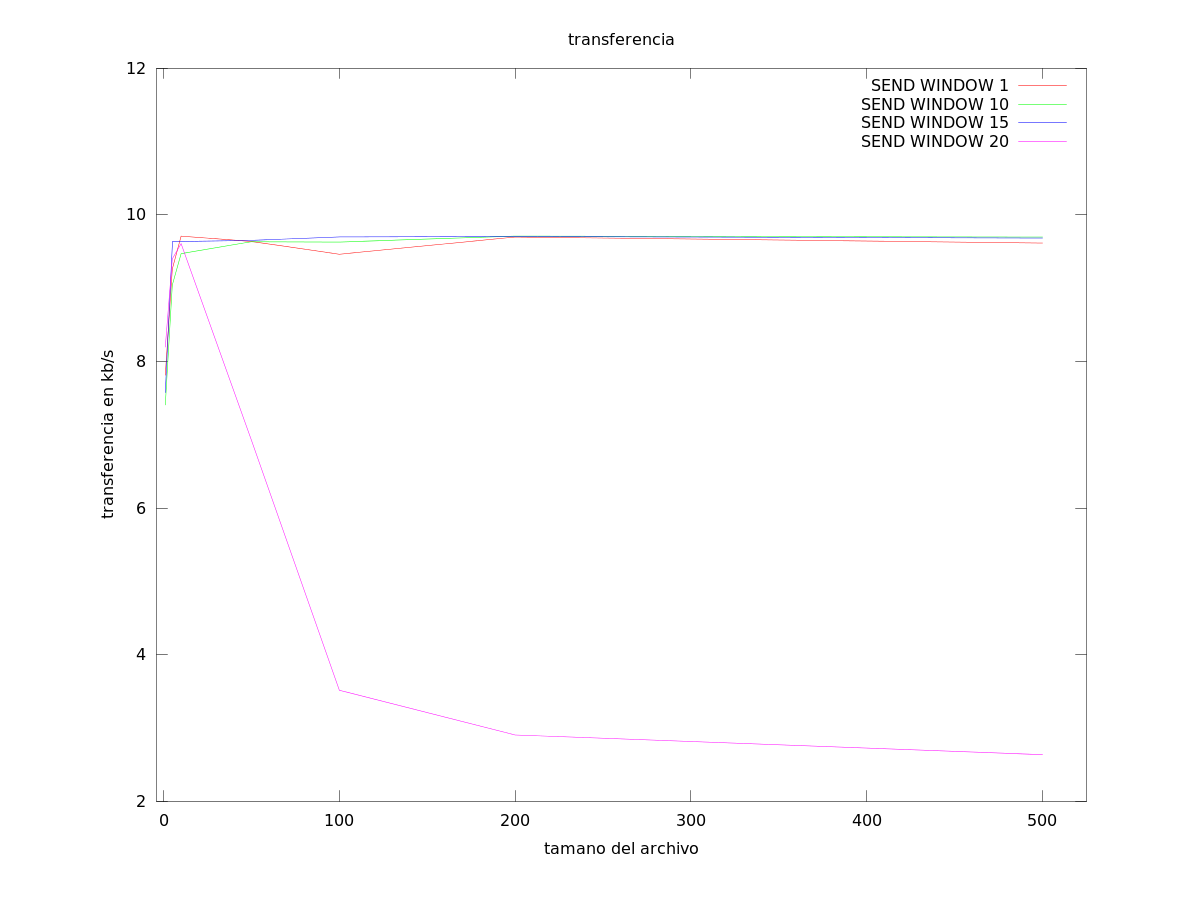
\includegraphics[width=550pt]{./datos/transferencia.png}
          \caption{Tiempo de transmisión}
          \label{fig:vt}
\end{figure}

\clearpage

\subsection{Cantidad de TimeOut}
\indent En esta sección presentamos la cantidad de timeout que tuvieron en promedio el envió de los archivos.\\
Decidimos presentar esta información en forma de tabla para mejorar la visibilidad.\\
\begin{center}
   \begin{tabular}{| c | c | c | c | c |}
    \hline
    Tamaño del archivo/SEND\_WINDOW & 1 & 10 & 15 & 20\\
    \hline
    1kb & 0 & 0 & 0 & 0 \\
    \hline
    5kb & 0 & 0 & 0 & 0 \\
    \hline
    10kb & 0 & 0 & 0 & 0\\
    \hline
    50kb & 0 & 0 & 0 & 5\\
    \hline
    100kb & 0 & 0 & 0 & 14\\
    \hline
    200kb & 0 & 0 & 0 & 34\\
    \hline
    500kb & 0 & 0 & 0 & 94\\
    \hline
  \end{tabular}
\end{center}
